% \documentclass{beamer}
% \usetheme{Szeged}

% \begin{document}


%-------------------------------------------------------------------------------
%							SECOND SECTION
%-------------------------------------------------------------------------------
\section{Principe}

\subsection{Simulation de l'ETR}

\begin{frame}
  \frametitle{Le transfer radiatif}

Lorsque la photons se trouvent en presence de la matière, Trois phenomènes majeures (caratises par leurs opacites) se produisent:

\begin{columns}
  \begin{column}{0.5\textwidth}
    \footnotesize
   \begin{itemize}
     \item Emission ($\sigma_e$): Plus la temperature matiere est elevee, plus l'emission est importante % Typiquement on ne vas pas retrouver sigma_e dans nos equations car on va se placer dans l'ETL, et on Planck.
     \item Absorption ($\sigma_a$): Lorsqu'on est a l'equilibre thermique, $\sigma_a = \sigma_e$ % On va considerer en plus l'equilibre chimique ce qui donne l'ETL
     \item Scattering ($\sigma_c$): Il faut aussi tenir compte de la fonction de distribution angulaire de « scattering » $p(\bm{\Omega^\prime \rightarrow \bm{\Omega}})$.
   \end{itemize}
  \end{column}
  % \pause
  \begin{column}{0.5\textwidth}
     \begin{center}
      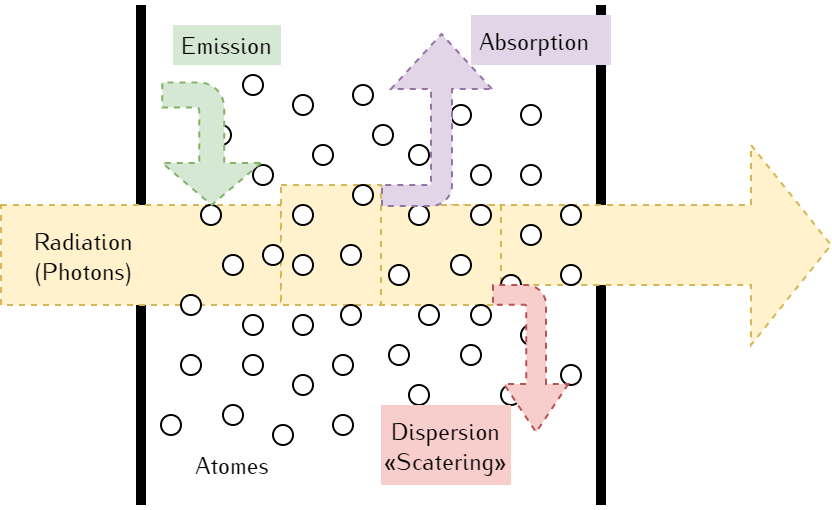
\includegraphics[width=6cm]{TransferRadiatif}       
     \end{center}
  \end{column}
 \end{columns}
 
\end{frame}

\begin{frame}
  \frametitle{L'ETR}
  L'equation du transfert radiatif est bilan d'energie lie au rayonnement au niveau mesoscopique. 

  \begingroup
  \scriptsize
  \begin{gather*}
      \begin{aligned}
      \frac{1}{c} \frac{\partial}{\partial t}I(t,\bvec{x},\bm{\Omega},\nu) &+\bm{\Omega}\cdot\nabla_{\bvec{x}} I(t,\bvec{x},\bm{\Omega},\nu) \\
      &= \sigma_a(\rho,\bm{\Omega},\nu)\left(B(\nu,T)-I(t,\bvec{x},\bm{\Omega},\nu)\right) \\
      &+ \frac{1}{4\pi} \int_{0}^{\infty} \int_{S^2}\sigma_c(\rho,\bm{\Omega},\nu)p(\bm{\Omega}^\prime\rightarrow\bm{\Omega})\left(I(t,\bvec{x},\bm{\Omega}^\prime,\nu)-I(t,\bvec{x},\bm{\Omega},\nu)\right) \, d\bm{\Omega}^\prime \, d\nu
      \end{aligned}
  % \label{eqn:ETR}
  \end{gather*}
  \endgroup
Où 
\begin{itemize}
  \item $I(t,\bvec{x},\bm{\Omega},\nu)$ designe l'intensité radiative specifique;
  \item $B(\nu,T)$ la fonction de Planck;
  \item $\oint p(\bm{\Omega}^\prime\rightarrow\bm{\Omega})\, d\bm{\Omega}^\prime=1$
\end{itemize}

\end{frame}

\begin{frame}
  \frametitle{Le modele P1}
  % Le modele P1: % Modèle macroscopique 5 aux moments (d’ordre 2), linéaire et hyperbolique. Le terme 1/3
  \begingroup
  \large
  \begin{equation*}
      \begin{cases}
       \partial_tE + c \ \operatorname {div} \bvec F = c\sigma_a\left(aT^4-E\right)\\
       \partial_t\bvec{F} + c \ \nabla E = -c\sigma_c \bvec{F} \\
       \rho C_v \partial_t T = c \sigma_a \left(E-aT^4\right)
      \end{cases}
  % \label{eqn:P1}
  \end{equation*}
  \endgroup
Ou:   % Moins precis que Monte-Carlo ou ordonne discretes; Mais plus rapide et suddisant; sigma
\begin{align*}
  E(t,\bvec{x}) &= \frac{4\pi}{c} \int_{0}^{\infty} \int_{S^2} I(t,\bvec{x},\bm{\Omega},\nu) \, d\bm{\Omega} \, d\nu \\
  \bvec{F}(t,\bvec{x}) &= \frac{4\pi}{c} \int_{0}^{\infty} \int_{S^2} \bm{\Omega}I(t,\bvec{x},\bm{\Omega},\nu) \, d\bm{\Omega} \, d\nu 
  % \label{eqn:EFT}
\end{align*}

\end{frame}

\begin{frame}
  \frametitle{Le schema de « splitting »: Etape 1}
  % Reglage de la temperature 
  \begin{columns}
    \begin{column}{0.5\textwidth}
      On pose $\Theta = aT^4$

      \begingroup
      \normalsize
      \begin{equation*} 
        \begin{dcases}
         E_j^{q+1} = \dfrac{\alpha E_j^n + \beta \gamma \Theta_j^n}{1 - \beta \delta} \\
         \Theta_j^{q+1} = \dfrac{\gamma \Theta_j^n + \alpha \delta E_j^n}{1 - \beta \delta} 
        \end{dcases}
    \label{eqn:Step1}
    \end{equation*}
      \endgroup
      En posant
      \scriptsize
      $\mu_q = \dfrac{1}{T^{3,n} + T^{n}T^{2,q} + T^{q}T^{2,n} + T^{3,q}}$
      \normalsize
      On a
    \end{column}
    % \pause
    \begin{column}{0.5\textwidth}
       \begin{center}
        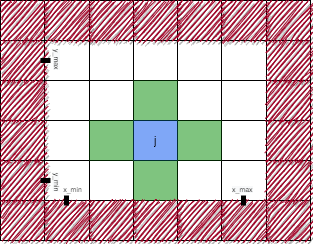
\includegraphics[width=4.5cm]{Dicretisation2D}       
       \end{center}
    \end{column}
   \end{columns}
   \tiny
  $\quad  \alpha = \dfrac{1}{\Delta t \left( \frac{1}{\Delta t} + c \sigma_a \right)} ,\quad 
   \beta = \dfrac{c \sigma_a}{\frac{1}{\Delta t} + c \sigma_a} ,\quad 
   \gamma = \dfrac{\rho_j C_v \mu_q}{\Delta t \left( \frac{\rho_j C_v \mu_q}{\Delta t} + c \sigma_a \right)} \quad \text{et} \quad  
   \delta = \dfrac{c \sigma_a}{\frac{\rho_j C_v \mu_q}{\Delta t} + c \sigma_a}.$

   \normalsize
   COnvergence ver $E_j^*$ et $\Theta_j^*$. $\bvec F_j$ reste constant egale a $F_j^*$.
   
\end{frame}


\begin{frame}
  \frametitle{Le schema de « splitting »: Etape 2}   % Adaptable aussi en 2D
  \begin{columns}
    \begin{column}{0.6\textwidth}
      \begingroup
      \normalsize
      \begin{equation*} 
          \begin{dcases}
          E_j^{n+1} = E_j^* + \alpha \sum_k \left( \bvec F_{jk}, \bvec n_{jk} \right) \\
          \bvec F_j^{n+1} = \beta \bvec F_j^* + \bm{\gamma} E_j^n + \delta \sum_k E_{jk} \bvec n_{jk}
          \end{dcases}   
      % \label{eqn:Step2}
      \end{equation*}
      Avec :
      % \begingroup
      \scriptsize
    
      % \begin{gather*}    
      % \begin{aligned} 
        $\alpha = -\frac{c \Delta t}{\left| \Omega_j \right|}, \linebreak
        \beta = \frac{1}{\Delta t} \left( \frac{1}{\Delta t} + c \sum_k M_{jk} \sigma_{jk} \right)^{-1}, \linebreak
        \bm{\gamma} = \frac{c}{\left| \Omega_j \right|} \left( \frac{1}{\Delta t} + c \sum_k M_{jk} \sigma_{jk} \right)^{-1} \left( \sum_k l_{jk} M_{jk} \bvec n_{jk} \right) \linebreak
        \delta = -\frac{c}{\left| \Omega_j \right|} \left( \frac{1}{\Delta t} + c \sum_k M_{jk} \sigma_{jk} \right)^{-1}$
    %   \end{aligned}
    % \end{gather*}

    \endgroup
      
    \end{column}
    % \pause
    \begin{column}{0.4\textwidth}
        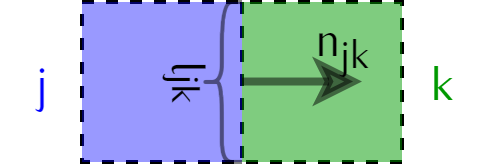
\includegraphics[width=5cm]{Interaction2D}       
       \begin{center}
        \begingroup
        \tiny
        \begin{align*}
          \left(\bvec F_{jk}, \bvec n_{jk} \right) &= l_{jk} M_{jk} \left( \frac{\bvec F_j^n \cdot \bvec n_{jk} + \bvec F_k^n \cdot \bvec n_{jk}}{2} - \frac{E_k^n - E_j^n}{2} \right) \\
          E_{jk} \bvec n_{jk} &= l_{jk} M_{jk} \left( \frac{E_j^n + E_k^n}{2} - \frac{\bvec F_k^n \cdot \bvec n_{jk} - \bvec F_j^n \cdot \bvec n_{jk}}{2} \right) \bvec n_{jk} \\
        %  \end{align*}
        %  \begin{align*}
          M_{jk} &= \frac{2}{2 + \Delta x \sigma_{jk}}  \\
          \sigma_{jk} &= \frac{1}{2} \left( \sigma_c(\rho_j,T_j^n) + \sigma_c(\rho_k,T_k^n) \right)
         \end{align*}
        \endgroup
       \end{center}
    \end{column}
   \end{columns}
\end{frame}

\subsection{L'architecture de reseau de neurones}

\begin{frame}
  \frametitle{Implementation C++}
  \begin{columns}
    \begin{column}{0.6\textwidth}
      \scriptsize
      \begin{itemize}
        \item Temps final = 0.01 \si{sh} %\textit{(1 shake (\si{sh}) = $10^{-8}$ secondes)}
        \item $c = 299$ [\si{\cm \per sh}]
        \item $a = 0.01372$ [\si{g \per cm \per sh^2  \per keV }]
        \item $C_v = 0.14361$ [\si{Jerk \per\g \per keV}] % \textit{(1 \si{Jerk} = 1\si{m \per \s\cubed})}
        \item La densité $\rho$ est un signal créneau [\si{\g\per\cm\cubed}]
        \item $\sigma_a = \rho T$ [\si{\per\cm}]
        \item $\sigma_c = \rho T$ [\si{\per\cm}]
        \item $T_0, T_{gauche} = 5$ [\si{keV}] % \textit{(en termes de température, 1 \si{keV} = 11605 \si{K})}
        \item $E_0 = aT_0^4$ [\si{g \per \cm \per sh^2}]
        \item $E_{gauche^*} = aT_{0}^4 + 5 \sin (2 k \pi t)$ [\si{g \per \cm \per sh^2}]
        \item $\bvec{F}_0, \bvec{F}_{gauche} = \bvec{0}$ [\si{g \per sh^2}]
        \item Sorties libres sur les autres bords
      \end{itemize}
    \end{column}
    % \pause
    \begin{column}{0.4\textwidth}
      %  \begin{center}
        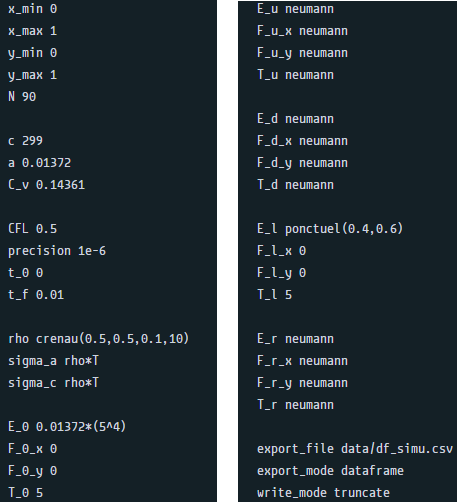
\includegraphics[width=4.5cm]{SimuCFG}   % EN 2D    
      %  \end{center}
    \end{column}
   \end{columns}
\end{frame}



% \end{document}
